%! Author = louis
%! Date = 28-10-22

Le projet ayant comme contrainte principale d'etre disponible sur toute les platformes majeur une base web me parait évident.
Pourtant, le web vient aussi avec la limitation pricipale qu'est le besoin de connection permanente au serveur,
pour remedier a ce probleme un PWA ( Application Web Progressive ) nous permetrais de beneficiez des avantages du web,
tout en permetant aux utilisateurs de concerver une version locale de l'application.
De plus une PWA permet d'etre instalée comme une application native Android ou IOS pour les platformes mobiles ce qui facilite l'accès.\\\\

Une PWA comme toute application web necesite plusieurs composant:
\begin{itemize}
    \item Un back-end
    \item une Base de Donnée
    \item une Interface definie pour le back-end ( API )
    \item un front-end
\end{itemize}
\subsubsection{TypeScript}
Pour ce projet j'ai decidé d'utiliser le meme language pour les 2 composant majeurs que sont le front et le back end.
Plusieurs choix s'offrais alors a moi , JavaScript, Kotlin, TypeScript ou n'importe quel language compilable en web assembly\\
JavaScript n'etait pas vraiment un bon choix vu qu'il ne propose pas de typage ce qui rend le code moin predictible et robuste.
Kotlin est un bon candidat il offre un typage statique mais propose de l'inference de type, peu etre transpiler vers du JavaScript ou du web assembly,
les outils de developement pour kotlin sont aussi tres bon mais la documentation pour une utilisation web est plutot pauvre comparer aux autres options.\\
TypeScript a quand a lui tout les avantage de Kotlin, grace au typage fort, et profite aussi de la documentation et des outil javaScript grave a ca nature de superset.
Lorsque l'on develope un produit web surtout pour un developeur Full Stack TypeScript est l'idéal.
Ces outils, l'enviromement JavaScript, la securité des Types et du null, la documentation.
Pour tout ces raison TypeScript est le language idéal pour le developement Web.
\subsection{Back-end}\label{subsec:back-end}
Le serveur back-end doit etre capable de mettre à disposition les données nécessaire au fonctionnement de l'application.
Cependant, le back-end sera aussi responcable des calculs d'équilibrage des dépenses, des matching de covoiturage et des trajets.\\\\
Connaissant deja Express.js et Spring ( Kotlin ) je me suis naturellement tourné vers ces derniers néanmoins je désirais utiliser du TypeScript pour ce projet.
Express.js est compatible avec TypeScript mais Spring ne l'est pas, Express.js est leger, minimaliste et propose une bonne documentation,
Spring est generaliste propose des outils de generation de code et utilise une systeme d'injection de dependance.
Ce qu'il me fallait etait une hybride entre Spring et Express.js.
Apres quelque recherche, j'ai trouvé un framework appler Nest.js, ce dernier supporte nativement TypeScript, propose une documentation ecxelante,
propose un CLI permetant de generer du code boiler-plate, reste simple et leger, Utilise de l'injection de dependance et est tres utiliser et apprecier par d'autre developeurs.
J'ai donc decider d'utiliser Nest.Js pour ce projet.

\subsubsection{ORM}
Nest.Js ( que je vais appeller Nest à partir de maintenant ) n'est pas un framework batteries included comme le son Spring ou Laravel,
Il m'a alors fallu choisir aussi un ORM pour interfacer avec ma base de donnée.
Dans la Documentation de Nest, il y a des exemples de configuration avec les ORM les plus Utiliser avec Nest et TypeScrip.
Ces derniers sont Sequelize, TypeOrm et Prisma,
ayant eu une experience avec Sequelize plus tot mauvaise lors de mon projet de dev3, j'ai decider de regarder du côté de prisma.
Prisma est une ORM un peu particulière dans le sens ou il propose d'utiliser une schema prisma pour definir ces entités plutôt que le code TypeScript.
Cella me paraissait une tres bonne chose vu que prisma generais alors lui meme les differents DTO nécessaire.
Il c'est cependant averer que a l'utilisation prisma n'est pas l'ideale surtout lorsque l'on désire le coupler à une API graphQl
À cause de son schema particulier, je devais definir le forma de mes entitée à 2 endroits et tout de meme crée manuelement mes DTO.
J'ai donc decider de jeter une oeuil à TypeOrm, celui-ci propose de definir les entités via des annotations TypeScript.
Ce qui me permet d'utiliser une seule classe pour definir mon entitée d'orm et de graphQl de plus TypeOrm est mieux
documenter grace au support d'une comunauter plus large.


\subsection{La base de donnée}\label{subsec:la-base-de-donnee}
Ma base de donnée devais me permetre 2 chose, stocker des données geographique et faire des operation sur ces données.
Le seul choix qui s'offrait à moi compatible avec TypeOrm etait postgress avec une extention nomer POSTGIS .
Postgres est une base de donnée tres utiliser en production et est tres performante et stable.

\subsubsection{Structure de donnée}
Pour stoquer tout les données nécessaire au fonctionnement de l'application, il nous faut une structure de donnée coherente.
Voici un shema de la base de donnée et de ca structure:
%Todo: Shema DB
\begin{figure}[ht]
    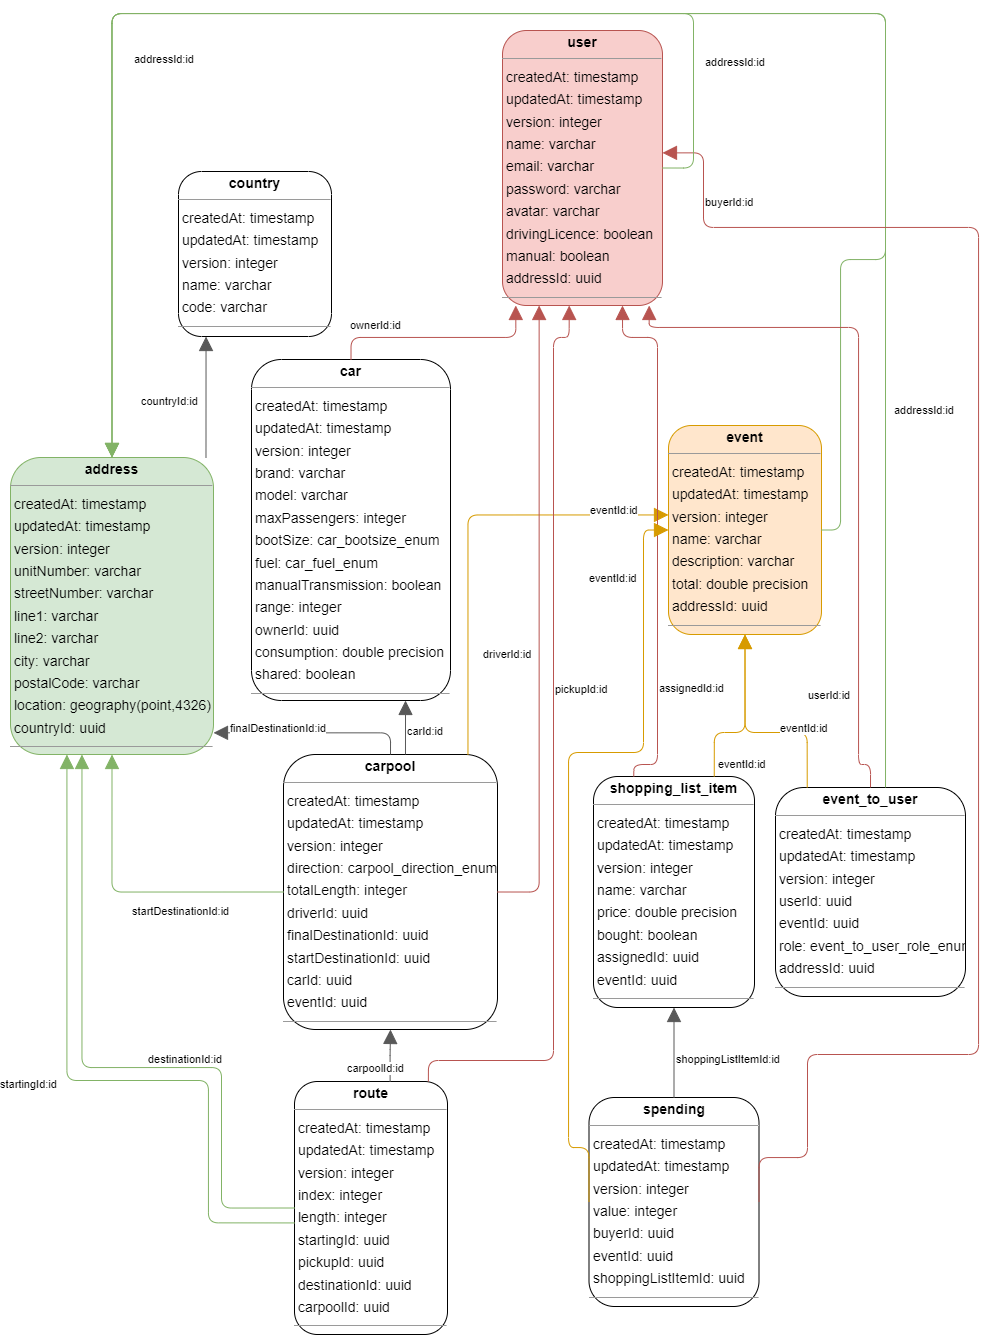
\includegraphics[width=\textwidth]{./images/dbShema}\caption{Architecture de la base de donnée}\label{fig:dbSchema}
    \centering
\end{figure}
\newpage

\subsection{L'API back end}\label{subsec:l'api-back-end}
Il existe plusieurs types d'API tres utiliser pour le Back-end mais les plus populaires sont le REST et le SOAP.
SOAP est de moin en moin utiliser dû à la complexité intrinsec du xml et à sa lourdeur.
Il nous reste donc REST qui est une bonne solution, mais nescecite pour presque chaque requete de recuperer des données qui ne seront pas toujour consomée par le client
Avec Rest l'on récupère une entitée complete tous les champs sont renvoyés.
C'est pour cela que graphQl a ete crée, non seulement graphQL utilise un typage fort via un schema defini et exposer par le serveur,
mais en plus graphql permet de ne recuperer que les champs nescesaire au client grace au GQL .




\subsection{Front-end}\label{subsec:front-end}
Pour ce qui est de l'interface utilisateur ( le front end ) j'ai decidé d'utiliser angular car ce framework utilise TypeScript nativement et supporte aussi les PWA
TypeScript est important, parce qu'il permet d'éliminer les bugs lier au typage d'objet avant meme l'execution du programe.
Angular etant un framework orienter m'oblige aussi à suivre une architecture propre qui permet de rendre independant les differents composants du projet.
